% =====================================================================
% VERSION ENSAE, REDUCTION SFE (phase 3, 1er octobre 2026) : chapitre 4, modele frequence-severite.
% Copie a texte constant de chapitres/06_socle_mecaniste.tex.
% Ne changent que les titres et les renvois repares, listes dans
% reduction/phase3.md.
% Lu par main_ensae.tex seul : ne jamais le faire lire par main_institut.tex,
% qui garde chapitres/.
% =====================================================================

\chapter{Modèle fréquence-sévérité}
\label{chap:socle}
\label{part:modele}

\noindent Le modèle combine une loi de sévérité de Pareto généralisée (GPD), commune à tous les
piliers touchés, et une loi de fréquence binomiale négative à dispersion posée.
La cascade du chapitre~\ref{chap:cascade} modifie seulement la façon dont ces deux
lois s'agrègent.

% MIGRÉ depuis memoire/main.tex (plages 787-932, 1492-1667).
% Hiérarchie descendue d'un cran, labels préfixés "soc:".
% RELECTURE FAITE (août 2026). Vérifié : aucune phrase de ce chapitre n'annonce la
% copule de Gumbel ni la variable latente comme LE modèle du mémoire ; la copule
% n'apparaît qu'au chapitre 13 comme axe de comparaison de la bande de modèle.
% Deux ambiguïtés de l'ancien modèle ont été levées ici :
%   (a) l'encadré "deux grilles coexistent" articule vecteur d'attaque et pilier ;
%   (b) l'encadré sur lambda_ref dit explicitement que les 341 de la PRC sont une clé
%       de répartition et n'alimentent PAS le moteur (l'entrée est lambda = 21,6).
% La charge systémique empirique a été corrigée sur la sortie réelle du script 08b
% (a = 0,122 [0,054 ; 0,223] ; phi = 2,24), l'ancien "a ~ 0,30 / phi ~ 3" était faux.
%--------------------------------------------------------------


\section{Théorèmes de l'extrapolation de queue}
% HARNAIS-HORS-SECTION: enonces de theoremes. Les nombres y sont des constantes d'enonce
%   (indices de domaine d'attraction, bornes, dates de publication), aucun n'est calcule
%   par le pipeline ; les valeurs empiriques correspondantes sont verifiees dans les
%   sections de calibration et de validation du meme chapitre.

\begin{theorem}[Fisher--Tippett--Gnedenko]\label{soc:th:ftg}
Soit $(X_i)_{i\ge1}$ i.i.d.\ de fonction de répartition $F$ et $M_n=\max(X_1,\dots,X_n)$. S'il existe des suites $a_n>0$, $b_n\in\R$ et une loi non dégénérée $H$ telles que $(M_n-b_n)/a_n \xrightarrow{d} H$, alors $H$ est, à un changement d'échelle et de position près, une loi des valeurs extrêmes généralisée (GEV) $H_\xi$. Le signe de $\xi$ détermine le domaine d'attraction : Fréchet ($\xi>0$, queue lourde), Gumbel ($\xi=0$) ou Weibull ($\xi<0$, support borné).
\end{theorem}

\noindent L'approche par maxima de blocs ne retient qu'une observation par bloc. Nous lui
préférons l'approche par dépassement de seuil, qui permet d'exploiter toutes les pertes au-delà d'un
seuil $u$. Celle-ci repose sur le théorème suivant, où
$G_{\xi,\sigma}(y)=1-\left(1+\xi y/\sigma\right)^{-1/\xi}$ désigne la loi de Pareto
généralisée (GPD).

\begin{theorem}[Pickands--Balkema--de Haan]\label{soc:th:balkema}
Soit $F$ dans le domaine d'attraction d'une GEV $H_\xi$ (Théorème~\ref{soc:th:ftg}). Alors il existe une fonction $\sigma(u)>0$ telle que la loi des excès converge uniformément vers une GPD lorsque le seuil approche la borne supérieure $x_F$ du support :
\begin{equation}
\lim_{u\to x_F}\ \sup_{0\le y< x_F-u}\bigl|F_u(y)-G_{\xi,\sigma(u)}(y)\bigr|=0,
\end{equation}
où $F_u(y)=\Prob(X-u\le y\mid X>u)$ et $G_{\xi,\sigma}$ est la fonction de répartition de la GPD. L'indice de queue $\xi$ est identique à celui de la GEV limite.
\end{theorem}

\noindent Pour $\xi>0$, la queue est lourde (figure~\ref{fig:domaines-attraction}). La variance de la
sévérité devient infinie dès $\xi\ge 1/2$, et son espérance dès $\xi\ge 1$ \citep{mcneil2015} :
avec $\hat\xi=0{,}595$ ci-dessous, la variance est infinie et l'espérance finie. Les énoncés développés
et les éléments de démonstration sont déportés \matcomp.

\section{Estimation de l'indice de queue}

% SOURCES-SCRIPTS: 47 63 67

L'estimateur de Hill étant biaisé hors du régime asymptotique strict, nous estimons la GPD par
maximum de vraisemblance sur les $N_u$ excès $y_i$ au-delà du seuil $u$. Pour $\xi \neq 0$, la
log-vraisemblance s'écrit
\begin{equation}
\ell(\xi, \sigma) = -N_u \ln(\sigma) - \left(1 + \frac{1}{\xi}\right) \sum_{i=1}^{N_u} \ln\left(1 + \frac{\xi y_i}{\sigma}\right)
\label{soc:eq:loglik-gpd}
\end{equation}
et se maximise numériquement par l'algorithme de Nelder-Mead. Par la delta-méthode, on obtient pour
l'indice de queue un intervalle de confiance asymptotique à $90\,\%$ égal à $[0{,}320\,;0{,}871]$,
qui recoupe l'intervalle bootstrap $[0{,}304\,;0{,}831]$.

% Figure ajoutee le 1er octobre 2026, demande de Kelian : tracee par le script 112, et non reprise
% d'un autre memoire. Les indices du panneau (a) et le -0,3 du panneau (b) sont des valeurs
% d'illustration ; seul l'indice calibre est un resultat, lu dans config.py par le script.
\begin{figure}[H]\centering
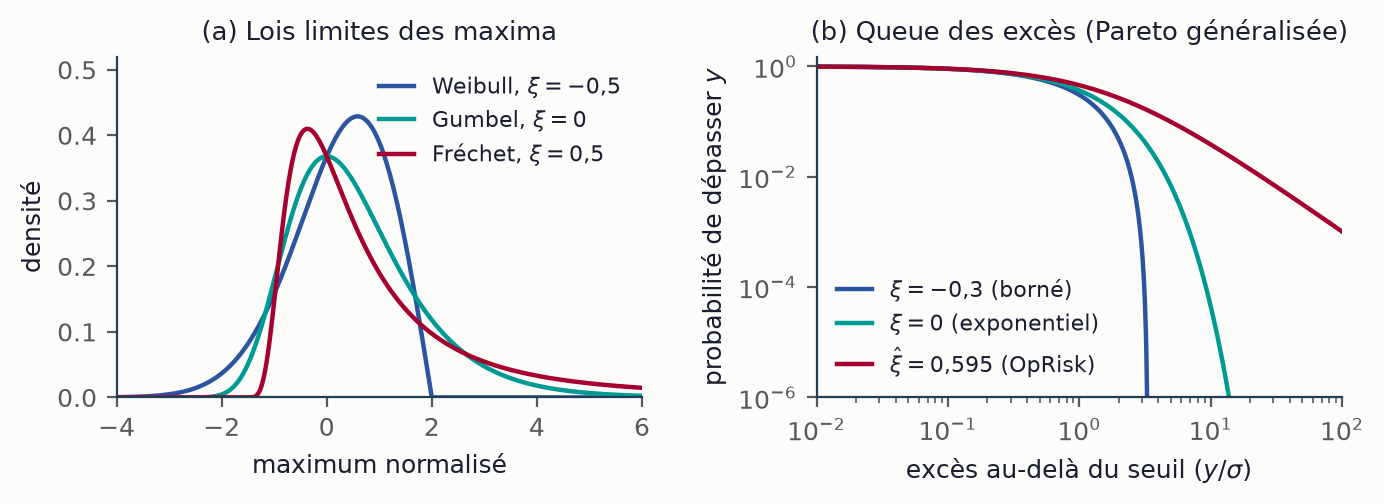
\includegraphics[width=0.95\textwidth]{GEV_domaines_attraction.png}
\caption{Domaines d'attraction des maxima et queue calibrée. (a) Densités des lois des valeurs
extrêmes généralisées de type Weibull ($\xi=-0{,}5$, support borné), Gumbel ($\xi=0$) et Fréchet
($\xi=0{,}5$, queue lourde), valeurs d'illustration. (b) Probabilité qu'un excès dépasse $y$ sous
une loi de Pareto généralisée d'échelle unité, en échelles logarithmiques. Les excès sont bornés
pour $\xi=-0{,}3$, et leur probabilité de dépassement décroît exponentiellement pour $\xi=0$, en
puissance pour l'indice calibré sur OpRisk, $\hat\xi=0{,}595$, qui relève du domaine de Fréchet.}
% SOURCES-SCRIPTS: 112
\label{fig:domaines-attraction}
\end{figure}

En notant $\zeta_u=\Prob(X>u)$, noté $p_u$ dans la suite, on dispose de formes fermées
classiques pour le quantile d'\emph{un} sinistre et sa moyenne de queue \citep{mcneil2015}. Ce
quantile n'est pas un besoin de capital, car celui-ci n'apparaît qu'après agrégation annuelle et
propagation dans la cascade.

\begin{proposition}[Quantile et moyenne de queue d'une sévérité GPD]\label{soc:prop:varestvar}
Sous le modèle POT, pour $\alpha$ tel que $\qsev_\alpha(X)>u$ et $\xi\in(0,1)$ :
\begin{align}
\qsev_\alpha(X) &= \boxed{\,u + \frac{\sigma}{\xi}\left[\left(\frac{1-\alpha}{\zeta_u}\right)^{-\xi}-1\right]\,},\label{soc:eq:var-gpd}\\[4pt]
\qbarsev_\alpha(X) = \E[X\mid X>\qsev_\alpha(X)] &= \boxed{\,\frac{\qsev_\alpha(X)}{1-\xi}+\frac{\sigma-\xi u}{1-\xi}\,}.\label{soc:eq:tvar-gpd}
\end{align}
Lorsque $\xi\ge 1$, l'espérance $\E[X]$ est infinie et $\qbarsev_\alpha$ n'est pas définie.
\end{proposition}

\noindent La calibration OpRisk ($u=20{,}03$, $\sigma=57{,}97$, $\xi=0{,}595$, $\zeta_u=0{,}151$)
donne par \eqref{soc:eq:var-gpd} un quantile de sévérité $\qsev_{99{,}5\%}(X)=663{,}0$~M\euro\ et
par \eqref{soc:eq:tvar-gpd} une moyenne de queue $\qbarsev_{99{,}5\%}(X)=1\,752{,}4$~M\euro. Ces
deux nombres décrivent un sinistre et ne se comparent jamais à un besoin de capital. Celui-ci est
$\VaR_{99{,}5\,\%}(L)$, quantile de la charge annuelle agrégée $L$, de l'ordre de plusieurs milliards
d'euros pour le périmètre financier étudié. Nous réservons $\VaR$ et $\TVaR$ à $L$,
$\qsev$ et $\qbarsev$ à $X$. À $\lambda\simeq21{,}6$ incidents enregistrés par an, l'approximation par perte unique associe au quantile annuel à $99{,}5\,\%$ un quantile
par sinistre de l'ordre de $99{,}98\,\%$. Les deux
échelles sont confrontées au \S\ref{sec:ancrage}.
% SOURCES-SCRIPTS: 67

Le vecteur d'attaque décrit l'entrée de l'incident : hameçonnage, exploitation de vulnérabilité
ou chaîne d'approvisionnement. Le pilier DORA désigne le contrôle qui a cédé.
Les parts $\pi_v$ des vecteurs répartissent la fréquence, sans appariement avec les piliers.
Le premier pilier touché suit les parts d'amorce du chapitre~\ref{chap:cascade} ; la cascade décrit la propagation qui suit.

\section{Loi de fréquence}

La fréquence de référence $\lambda_{ref}$ est lue sur le périmètre financier de la base PRC
($\lambda_{ref} = 341$ notifications/an). Nous la décomposons en sous-fréquences par vecteur
d'attaque, selon la structure de la base Hackmageddon :
% SOURCES-SCRIPTS: 62
\begin{equation}
\lambda_{ref} = \sum_{v} \lambda_v,
\qquad
\lambda_v = \lambda_{ref} \times \pi_v,
\end{equation}
où $\pi_v$ est la part du vecteur $v$ ($38{,}8\,\%$ hameçonnage, $33{,}8\,\%$ exploitation de
vulnérabilités, $15{,}8\,\%$ chaîne d'approvisionnement, $6{,}3\,\%$ identifiants compromis, $5{,}3\,\%$
autres). Un
défaut de conformité sur une exigence n'agit ainsi que sur la sous-fréquence du vecteur qu'elle
atténue. Les $341$ notifications américaines, sans seuil de matérialité, ne servent qu'à cette décomposition par vecteur. La base entière en compte $2\,150$ par an. L'entrée du
moteur est la fréquence conventionnelle des événements TIC collectés par OpRisk, $\lambda \simeq 21{,}6$ par an
pour le périmètre financier étudié, et tout niveau de capital du chapitre~\ref{chap:resultats}
repose sur elle.

Afin de tenir compte de la surdispersion ($\sigma^2/\mu > 1$), nous modélisons la fréquence agrégée
$\lambda_{S_x} = \lambda_{\text{C}}\sum_v \pi_v\, m_{v,S_x}$ d'un scénario $S_x$ par une loi binomiale
négative. Nous attribuons à l'état conforme la fréquence historique $\lambda_{\text{C}}\simeq 21{,}6$.
C'est une hypothèse, car aucune base n'observe l'état de conformité.
Nous posons $\phi = \sigma^2/\mu = 9{,}2$, constant d'un scénario à l'autre, et le paramètre
$r$ est recalculé :
\begin{equation}
r_{S_x} = \frac{\lambda_{S_x}}{\phi - 1},
\qquad
p_{S_x} = \frac{r_{S_x}}{r_{S_x} + \lambda_{S_x}}.
\end{equation}
La surdispersion en régime de forte dégradation n'est pas observée, faute
d'historique de crise DORA.

Pour un mélange de Poisson, l'indice de dispersion $1+\lambda/r$ croît avec la fréquence à $r$ fixé.
Le moteur maintient $\phi$ constant et recalcule $r$. L'indice est de $1{,}19$ sur les $14\,944$ cellules firme-année du
panel, de $2{,}24$ sur la série annuelle sectorielle détendancée (IC~$95\,\%$ $[1{,}24\,;5{,}18]$,
dix-huit points), et nous retenons $9{,}20$ dans le moteur.

Cette dernière valeur est un choix de prudence sur la queue de fréquence, pas une calibration. Il
en va de même de la charge systémique $a=0{,}60$ du mélange de la fréquence (supplément), qui dépasse la
borne haute de l'intervalle de la charge empirique $a=0{,}122$ (IC~$95\,\%$ $[0{,}054\,;0{,}223]$).
La charge $a$ est le coefficient du facteur dans le mélange lognormal $\exp(aY-a^2/2)$. Passer du Poisson à la
binomiale négative posée relève le besoin de capital du périmètre financier étudié de $+9\,\%$, la queue
restant déterminée au $99{,}5\,\%$ par la perte unique dominante.
% SOURCES-SCRIPTS: 47 08b 67 41

Le moteur tire indépendamment les comptes annuels selon cette loi binomiale négative.
Le facteur commun de conformité $\Theta$ intervient dans les probabilités des états C, PC et NC
(chapitre~\ref{chap:multietats}), auxquels correspondent les scénarios $S_0$, $S_1$ et $S_2$.
Les capitaux publiés sont calculés dans ces états discrets.

\section{Loi de sévérité}
\label{soc:sec:severite}

Chaque pilier touché reçoit une sévérité élémentaire : zéro avec probabilité $1-p_u$, ou $u+Y$, avec $Y$ de loi GPD.
Les pertes sous le seuil sont négligées. La perte d'un incident est la somme de ces sévérités,
hypothèse d'additivité non testée faute de coûts observés par pilier. La fréquence compte les événements avant ce tirage.

% SOURCES-SCRIPTS: 07 47 63 67

Sur la population OpRisk de fréquence et de descente d'échelle, les $10\,\%$ d'incidents les plus graves concentrent $92{,}3\,\%$ de la perte totale
(chapitre~\ref{chap:donnees}), ce qui conduit à représenter la queue par une GPD au-delà d'un seuil $u$
(\emph{peaks-over-threshold}). Au seuil du percentile~85 ($u = 20{,}0$~M\euro, 91 excès) :
\begin{equation}
\hat{\xi}_{\text{OpRisk}} = 0{,}595 \quad (\text{IC}_{90\%}=[0{,}30\,;\,0{,}83]),
\qquad
\hat{\sigma}_{\text{OpRisk}} = 58{,}0~\text{M\euro},
\qquad
\qsev_{99{,}5\%}(X) = 663~\text{M\euro}.
\end{equation}
L'intervalle bootstrap du quantile de sévérité, $[411\,;\,1037]$~M\euro, représente un facteur~2{,}5
entre les bornes, dû à la seule incertitude de paramètre. Nous plaçons le seuil là où l'indice de
forme quitte la zone $\xi \geq 1$, dans laquelle l'espérance n'existe pas, tout en gardant assez
d'excès pour l'estimation ($n = 91 > 30$). Cet argument ne tient qu'au voisinage du seuil, l'indice
décroissant sur toute la plage (\S\ref{soc:sec:validation}).

\section{Estimateur de Hill}

% SOURCES-SCRIPTS: 47 63 67

Au seuil retenu ($k=86$), l'estimateur de Hill \citep{Hill1975} atteint $1{,}32$ et dépasse de
$120{,}8\,\%$ le maximum de vraisemblance. Sur $2\,000$ échantillons simulés sous le modèle publié,
les six valeurs observées de Hill tombent dans l'intervalle simulé à $90\,\%$, si bien que l'écart
correspond à celui qu'un indice de $0{,}595$ produit en échantillon fini. De plus, Hill croît avec $k$ alors que
le balayage de seuil fait décroître $\hat\xi$, ce qui serait inversé si la queue valait $1{,}32$.
Sur la PRC, $\hat\xi = 1{,}03$ concerne un autre objet, puisque la sévérité y est une puissance du
nombre d'enregistrements (\S\ref{sec:oprisk}).

\section{Adéquation des lois}
\label{soc:sec:validation}

Pour la sévérité, les tracés quantile-quantile et probabilité-probabilité s'alignent sur la
diagonale, et la vie résiduelle moyenne est linéaire au-delà du seuil (figure~\ref{soc:fig:validation}).
L'estimation $\hat\xi$ est stable à $0{,}5\,\%$ près au voisinage du seuil retenu, jusqu'au
percentile $85$ des données courantes. Du percentile $85$ au percentile $95$, elle décroît de
$0{,}60$ à $0{,}38$ sur quatre seuils comptant chacun au moins trente excès, sans sortir de
l'intervalle à $90\,\%$ publié, $[0{,}30\,;0{,}83]$. Sous le seuil retenu, elle remonte jusqu'à
$0{,}98$ et sort de cet intervalle, ce qui traduit le biais de seuil attendu et interdit de
descendre plus bas.

Les tests par bootstrap paramétrique (91 excès) ne rejettent ni la famille GPD (Anderson-Darling $p=0{,}96$,
écart de Kolmogorov-Smirnov mesuré aux seuls points d'observation, $p=0{,}89$), ni le couple $(\hat\xi,\hat\sigma)$ publié, paramètres imposés
(Anderson-Darling $p=0{,}99$, Kolmogorov-Smirnov $p=0{,}89$). Mesurée par simulation, la couverture
réelle de l'intervalle à $90\,\%$ de $\xi$ est de $86\,\%$, donc l'intervalle est trop
étroit et l'élargir d'environ $10\,\%$ rétablirait le nominal. La sous-couverture concerne l'incertitude de l'estimation ; elle n'établit pas le signe d'un biais du capital. Le taux de dépassement et la dérive d'échelle font l'objet de diagnostics distincts (\S\ref{sec:pu-coherence} et \S\ref{soc:sec:backtest}).

Le test du rapport de vraisemblance rejette le Poisson au profit de la binomiale négative (statistique $130{,}5$, $p\approx 10^{-30}$ sur $14\,944$ cellules firme-année), bien que $\Var/\E=1{,}19$ reste proche de un. Ce $p$ traite les cellules comme indépendantes et ignore la dépendance par firme ; le rejet ne calibre pas non plus le facteur $9{,}2$ du moteur.

\begin{figure}[H]\centering
\figover{J3_validation_adequation.png}
\caption{Adéquation du socle. (a-b) Diagrammes quantile-quantile et probabilité-probabilité de la sévérité
contre la GPD ajustée. (c) vie résiduelle moyenne, linéaire au-delà de $u$. (d) stabilité
de $\hat\xi$ au seuil. (e) test d'Anderson-Darling, loi nulle par bootstrap
paramétrique et statistique observée ($p=0{,}96$). (f) adéquation de la fréquence :
la binomiale négative colle aux comptes firme-année, le Poisson rate la queue.}
% SOURCES-SCRIPTS: 47 93
\label{soc:fig:validation}
\end{figure}

Une règle de stabilité appliquée à dix percentiles candidats retient $19{,}87$~M\euro{} contre
$20{,}03$ publiés, avec un quantile identique. Ce seuil est également le mieux ajusté du balayage.
La règle la plus permissive descendrait à $12{,}88$~M\euro{} et donnerait un quantile de sévérité
supérieur de $16{,}0\,\%$.

Lorsqu'on retire chacun des $91$ excès à son tour, le quantile de sévérité balaie une étendue de
$111{,}7$~M\euro, qui représente $17{,}9\,\%$ de l'amplitude de l'intervalle publié, sans jamais en
sortir. Le plus gros excès, $1\,380$~M\euro, le déplace de $-15{,}8\,\%$. Sur le périmètre
calibré, le maximum équivaut à $3{,}7$ fois le quantile à $99\,\%$, contre $52{,}7$ sur la base
entière.

Retirer les trois plus grosses pertes ramène le quantile sous la borne basse.
En retirer cinq le fait passer de $657{,}2$ (quantile recompté, contre $662{,}78$ publié) à $327{,}3$~M\euro.
L'indice $\xi$ passe alors de $0{,}60$ à $0{,}22$.
Le quantile publié dépend donc de ces quelques pertes. Ces tests portent sur la forme des lois, non sur le niveau du capital.
% SOURCES-SCRIPTS: 106 41

\section{Backtest hors échantillon}
\label{soc:sec:backtest}

Pour chaque année d'origine, nous ajustons les deux lois sur les seules observations antérieures et
évaluons la prévision de l'année suivante, puis l'origine avance d'un an. La fenêtre va de $2004$ à $2025$
($539$ incidents, douze années notées), car avant $2004$ la base compte de un à neuf incidents par
an, et $2026$ n'en compte que cinq. Le seuil est ré-estimé sur chaque échantillon d'apprentissage
par la règle du percentile $85$.

Un intervalle de prévision à $90\,\%$ contient la réalisation $11$ années sur $12$ ($91{,}7\,\%$)
sous la binomiale négative et $9$ sur $12$ ($75{,}0\,\%$) sous le Poisson. Le log-score cumulé de la binomiale négative dépasse celui du Poisson de $3{,}054$ nats, gain dû à trois années. Douze années donnent trop peu de puissance : ce
résultat va dans le sens du choix de la binomiale négative sans le démontrer, et il ne teste pas
le facteur de surdispersion posé dans le moteur. Le test de Kolmogorov-Smirnov sur la probabilité intégrale
des excès ne rejette pas la GPD ($D=0{,}100$, $p=0{,}4087$), avec peu d'excès donc peu de
puissance. Le test de Kupiec rejette la couverture des quantiles de sévérité à $99\,\%$
($p=0{,}0078$) et à $99{,}5\,\%$ ($p=0{,}0140$), avec $8$ et $5$ dépassements pour $2{,}8$ et
$1{,}4$ attendus. L'échelle de la queue dérive de $4{,}00\,\%$ par an, dont la moitié
d'inflation monétaire. L'effet sur le quantile de sévérité est
d'au moins $+24{,}7\,\%$.

Sous la sévérité dérivée, le facteur entre états (rapport des capitaux non conforme sur conforme, chapitre~\ref{chap:resultats}) passe de
$3{,}344$ à $3{,}124$ ($-6{,}6\,\%$) et l'écart en euros bouge de $-1{,}9\,\%$, par compensation
entre forme et échelle. La charge annuelle agrégée est rejetée pour la même cause, sur les dernières
années notées seulement. L'indépendance entre fréquence et sévérité tient sur les excès. Ce
défaut d'échelle figure au registre des limites (\S\ref{sec:pu-coherence}), et nous ne corrigeons
pas la valeur publiée.
% SOURCES-SCRIPTS: 89 90 91 102

Détecter un doublement du taux de dépassement avec $80\,\%$ de puissance demanderait $1\,811$ années à $99{,}5\,\%$, $905$ à $99\,\%$ et $78$ à $90\,\%$. Douze années ne valident donc pas la queue du capital.
